% !TeX spellcheck = cs_CZ
%======== Kapitola: Konstrukce vypínačů pro VN a VVN ===============================================
\chapter{Konstrukce vypínačů pro VN a VVN}
\minitoc

%  \section{Vypínače olejové a máloolejové}
%  \section{Tlakovzdušné vypínače}
%  \section{Tlakoplynové vypínače}
%  \section{Vakuové vypínače}
  \section{Tlumící rezistory pro vypínače}
    Po vypnutí proudu vzrůstá mezi kontakty vypínače \emph{zotavené napětí}. Strmost vzrůstu zotaveného napětí v počáteční fázi je velmi častou příčinou selhání vypínače, což platí zejména při vypínání blízkého zkratu. Při velkých strmostech zotaveného napětí, zejména při velkých vypínacích proudech, nejsou často již možné další konstrukční úpravy zhášecí komory ke zvětšení vypínací schopnosti. Řazení nepřiměřeně velkého počtu zhášecích komor do série 
    komplikuje značně celý vypínač, i když se tímto řešením mohou zvládnout požadované vysoké parametry. Hledají se tedy jiná "rozumná" řešení vedoucí ke zmenšení počáteční strmosti zotaveného napětí. Prvním řešením je úprava sítě např. připojením kondenzátoru k vypínači, což bylo v některých případech i realizováno. Kondenzátory však vycházejí pro napětí vvn příliš velké a nákladné. Jiný způsob zvětšení kapacity vedení je připojení vypínače ke kabelu. 
    To se používá u zapouzdřených rozvoden pro napětí 123 kV ve městech, kde je kabel nutný i ze stavebních důvodů. Pro rozvodny připojené k venkovnímu vedení je použití kabelu nevhodné a drahé. Vypínače v rozvodnách ve volném terénu jsou připojeny k venkovnímu vedení a zmenšení strmosti zotaveného napětí na svorkách vypínače se řeší u tlakovzdušných vypínačů použitím \textbf{tlumících rezistorů} připojeného paralelně ke svorkám vypínače. Tlumící rezistor je organickou součástí vypínače a po vypnutí hlavní zhášecí komory se pak proud jdoucí rezistorem následně vypíná pomocným zhášedlem. Pro zvláště vysoká napětí (nad 420 kV) slouží tlumící rezistor také k omezení zapínacího přepětí.

    \begin{figure}[ht!]
      \centering
      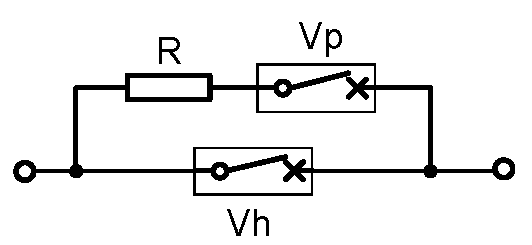
\includegraphics[scale=0.6]{tlumici_rezistor_zhasedlo.pdf}
      \caption[Schéma spínací jednotky vypínače s tlumícím rezistorem.]{Schéma spínací jednotky    
              vypínače s tlumícím rezistorem.($V_h\cdots$ hlavní zhášecí komora, $V_p\cdots$ 
              pomocný spínač, $R \cdots$ tlumící rezistor.)}
      \label{epr:fig_tlum_res}
    \end{figure}
    Uvedené dva důvody jsou v současné době rozhodující pro používání tlumících rezistorů. U vypínačů s malou rychlostí deionizace vypínací dráhy se používal tlumící rezistor i pro zamezení přepětí v důsledku elektrických průrazů při vypínání kapacitních proudů. Dalším důvodem použití tlumících rezistorů je omezení přepětí při vypínání malých indukčních proudů, jako např. u transformátorů naprázdno.

    Pro každý uvedený důvod použití tlumících rezistorů jsou jiná kritéria na volbu odporu rezistoru. Na obr. \ref{epr:fig_tlum_res} je příkladné schéma vypínací jednotky s tlumící rezistorem v zapnuté poloze.
    \begin{itemize}
      \item Postup při vypínání: vypne hlavní zhášecí komora $V_h$ $\Rightarrow$ vypne pomocný vypínač $V_p$.
      \item Postup při zapínání s tlumícím rezistorem: zapne pomocný spínač $V_p$ $\Rightarrow$ zapne hlavní zhášecí komora $V_h$.
      \item Při spínání je časové řízení spínání voleno tak, aby bylo vždy mezi jednotlivými spínacími operacemi zaručeno vypnutí, tj. přerušení
      proudu a uhasnutí oblou\-ku ve zhášecích komorách.
    \end{itemize}

   Použití tlumícího rezistoru vždy poněkud komplikuje konstrukci vypínače, ale zase snižuje nároky 
   na dimenzování hlavní zhášecí komory vypínače. Je nutné vždy uvážit použití tlumícího rezistoru 
   a volit jeho optimální odpor.

%---------------------------------------------------------------------------------------------------
% \printbibliography[heading=subbibliography]
\addcontentsline{toc}{section}{Seznam literatury}
